%%%%%%%%%%%%%%%%%%%%%%%%%%%%%%%%%%%%%%%%%
% University/School Laboratory Report
% LaTeX Template
% Version 3.0 (4/2/13)
%
% This template has been downloaded from:
% http://www.LaTeXTemplates.com
%
% Original author:
% Linux and Unix Users Group at Virginia Tech Wiki 
% (https://vtluug.org/wiki/Example_LaTeX_chem_lab_report)
%
% License:
% CC BY-NC-SA 3.0 (http://creativecommons.org/licenses/by-nc-sa/3.0/)
%
%%%%%%%%%%%%%%%%%%%%%%%%%%%%%%%%%%%%%%%%%

%----------------------------------------------------------------------------------------
%	PACKAGES AND DOCUMENT CONFIGURATIONS
%----------------------------------------------------------------------------------------

\documentclass{article}

\usepackage[version=3]{mhchem} % Package for chemical equation typesetting
\usepackage{siunitx} % Provides the \SI{}{} command for typesetting SI units

\usepackage[top=1in, bottom=1in, right=1in, left=1in]{geometry}

%Add code formating
\usepackage{listings}
\lstset{tabsize=2}

\usepackage{hyperref}

\usepackage{amssymb}

\usepackage{enumerate}

\usepackage{multicol} % Multi-column support

\usepackage{enumitem}

%Add extra support for image placement
\usepackage{float}

\usepackage{mcode}

\usepackage{graphicx} % Required for the inclusion of images

\setlength\parindent{0pt} % Removes all indentation from paragraphs

\renewcommand{\labelenumi}{\alph{enumi}.} % Make numbering in the enumerate environment by letter rather than number (e.g. section 6)

%\usepackage{times} % Uncomment to use the Times New Roman font

%----------------------------------------------------------------------------------------
%	DOCUMENT INFORMATION
%----------------------------------------------------------------------------------------

\title{Keysight Hacking Platform Hardware Overview} % Title

\author{Blake \textsc{Vermeer}} % Author name

\date{\today} % Date for the report

\begin{document}

\maketitle % Insert the title, author and date

\begin{center}
\begin{tabular}{l r}
Date Performed: & March 26, 2017 \\ % Date the experiment was performed
Company: & Keysight Technologies % Company
\end{tabular}
\end{center}

% If you wish to include an abstract, uncomment the lines below
% \begin{abstract}
% Abstract text
% \end{abstract}

%----------------------------------------------------------------------------------------
%	OVERVIEW
%----------------------------------------------------------------------------------------
\section{Overview}

This document gives an overview of the available GPIO lines and interfaces. It also explains how these different interfaces can be enabled and used.


%----------------------------------------------------------------------------------------
%	RPi 3 Block Diagram
%----------------------------------------------------------------------------------------
\section{Raspberry Pi 3 Block Diagram}

	\begin{minipage}{0.5\textwidth}
		
		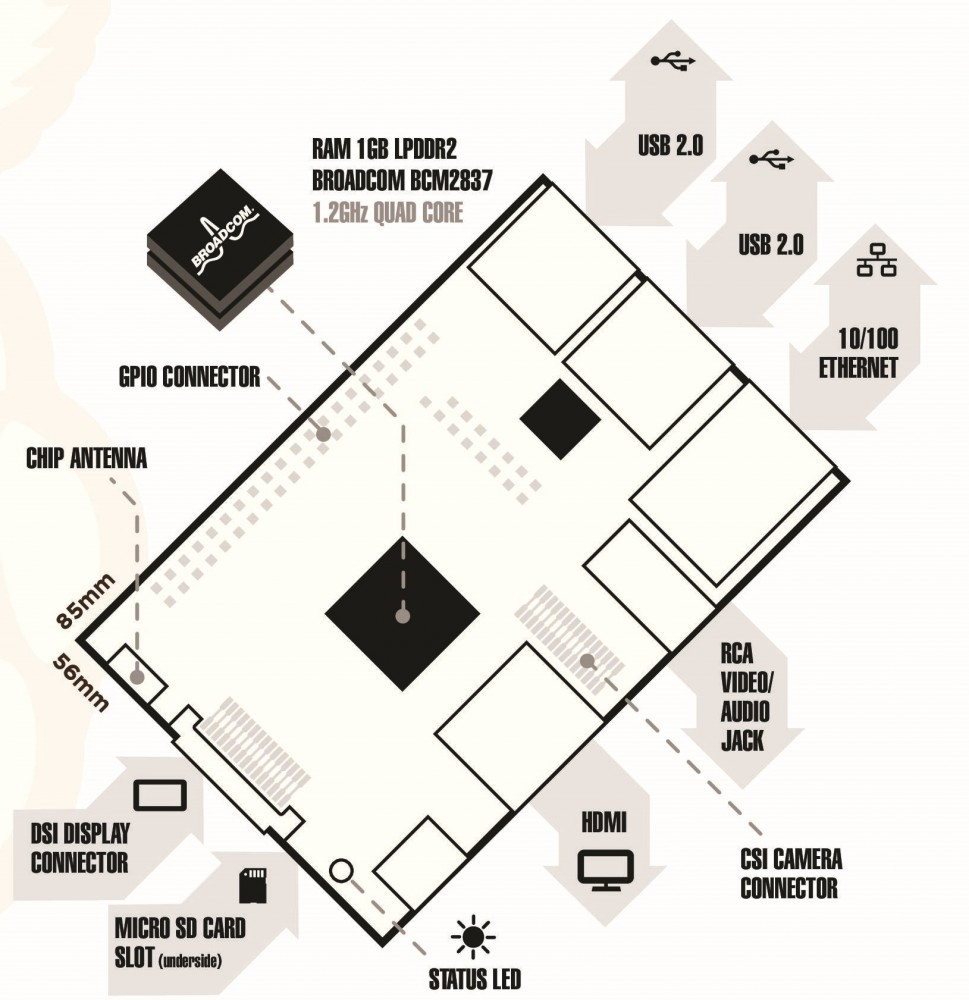
\includegraphics[width=0.95\textwidth]{pics/Raspberry-Pi-3_Block_Diagram.jpg}
		
		%\begin{figure}[H]
		%	\centering
		%	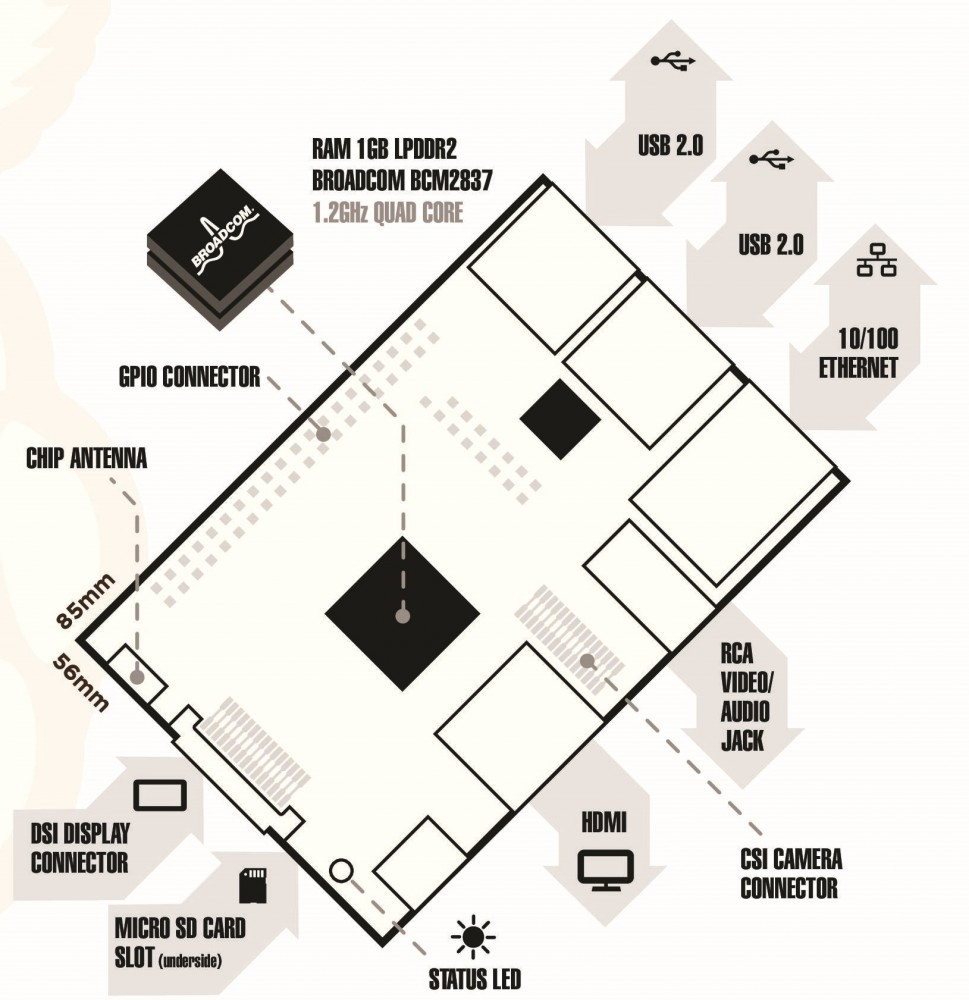
\includegraphics[scale=0.3]{pics/Raspberry-Pi-3_Block_Diagram.jpg}
		%	\caption{Raspberry Pi 3 Block Diagram}
		%	\label{RPi_3_Block_Diagram}
		%\end{figure} 
	
	\end{minipage}
	\begin{minipage}{0.45\textwidth}
		
		\begin{itemize}
			\item CPU: 1.2 GHz quad-core ARM Cortex A53
			\item Memory: 1 GB LPDDR2-900 SDRAM
			\item 4 USB ports (Max current draw of 1.2A combined on all the USB ports)
			\item 10/100 Ethernet
			\item HDMI
			\item Bluetooth 4.0
			\item 802.11n Wireless LAN
		\end{itemize}
	
	\end{minipage}








%----------------------------------------------------------------------------------------
%	RPi 3 GPIO Usage Overview
%----------------------------------------------------------------------------------------
\section{Raspberry Pi 3 Used GPIO Lines}




%----------------------------------------------------------------------------------------
%	RPi 3 Available GPIO and Interfaces
%----------------------------------------------------------------------------------------
\section{Raspberry Pi 3 Available GPIO and Interfaces}




%----------------------------------------------------------------------------------------
%	APPENDIX
%----------------------------------------------------------------------------------------

%\newpage
%\section{Appendix}

%\begin{enumerate}

	
%	\item[1. a.)] \lstinputlisting{../MATLAB/problem_1a.m}
	

%\end{enumerate}






%----------------------------------------------------------------------------------------


\end{document}